\section{Complications}

[I have a note: TC1: Track local state ???]

\subsection{Release Acquire}

Can be encoded in independency, or logic, but logic is compatible with fork.

Logic is also more flexible, and we need that for \armeight.

We use $\Q$.

\begin{definition}
  $\aPS$ is \emph{completed} if $\aTr[\aEvs](\Q)$ implies $\Q$.
\end{definition}


\subsection{Coherence}

$\Q[\mSC]$ implies $\Q[\mRA]$ implies $\Qx{\aLoc}$ implies $\Qw{\aLoc}$

Can be encoded in independency, or logic.

If you put in independency then you add this to $\sSTORE{}{}$:
\begin{itemize}
\item if $\bEv\in\aEvs_1$ and $\aEv\in\aEvs_2$ either $\bEv<\SB0\aEv$ or $a\reorder\labeling_2(\aEv)$.
\end{itemize}
This does not do the right thing with fork however.  If you want to enforce
coherence this way then you need to use fork-join as the sequential
combinator, rather than fork.

Instead we put it in the logic, using 

\begin{itemize}
\item Coherence respects program order: $\Qx{\aLoc}$
\item Drop read-read coherence: $\Qw{\aLoc}$ (Required for CSE without
  alias analysis over read only code, not required by hardware)
\end{itemize}



\subsection{ARM Compilation: Internal Acquires}
Downgrading acquires/Anton example: $\Dx{\aLoc}$

\subsection{ARM Compilation: Read-read dependencies}
$\RW$/$\RO$ (control dependencies into reads as in MP with
release on right and control dependency on left)

\subsection{Redundant Read Elimination}

Requires indexing to resolve nondeterminism.

\begin{gather*}
  \taglabel{TC2}
  \PR{x}{r}\SEMI
  \PR{x}{s}\SEMI
  \IF{r{=}s}\THEN \PW{y}{1}\FI
  \PAR
  x\GETS y
  \\
  \hbox{\begin{tikzinline}[node distance=1.5em]
  \event{a1}{\DR{x}{1}}{}
  \event{a2}{\DR{x}{1}}{right=of a1}
  \event{a3}{\DW{y}{1}}{right=of a2}
  % \po{a2}{a3}
  % \po[out=-20,in=-160]{a1}{a3}
  \event{b1}{\DR{y}{1}}{right=3em of a3}
  \event{b2}{\DW{x}{1}}{right=of b1}
  \rf{a3}{b1}
  \po{b1}{b2}
  \rf[out=169,in=11]{b2}{a2}
  \rf[out=169,in=11]{b2}{a1}
    \end{tikzinline}}
\end{gather*}
Precondition of $\DWP{y}{1}$ is $(r{=}s)$ in
\begin{math}
  \sem{\IF{r{=}s}\THEN y\GETS 1\FI}.
\end{math}
Predicate transformers for $\emptyset$ in $\sem{\PR{x}{r}}$ and $\sem{\PR{x}{s}}$ are
\begin{align*}
  \PREDP{(r{=}1 \lor r{=}x)\limplies\aForm[r/x]},
  \\
  \PREDP{(s{=}1 \lor s{=}x)\limplies\aForm[s/x]}.
\end{align*}
Combining the transformers, we have
\begin{displaymath}
  \PREDP{(r{=}1 \lor r{=}x)\limplies(s{=}1 \lor s{=}r)\limplies\aForm[s/x]}.
\end{displaymath}
Applying this to $(r{=}s)$, we have
\begin{displaymath}
  \PREDP{(r{=}1 \lor r{=}x)\limplies (s{=}1 \lor s{=}r)\limplies (r{=}s)},
\end{displaymath}
which is not a tautology.

Same problem occurs oopsla, where we have:
\begin{align*}
  \PREDP{\aForm[v/x,r] \land \aForm[x/r]},
  \\
  \PREDP{\aForm[v/x,s] \land \aForm[x/s]}.
\end{align*}
Combining the transformers, we have
\begin{displaymath}
  \PREDP{\aForm[v/x,r,s] \land \aForm [v/x,r][x/s] \land \aForm[x/r][v/x,s] \land \aForm[x/r,s]}.
\end{displaymath}
Applying this to $(r{=}s)$, we have
\begin{displaymath}
  \PREDP{v{=}v \land v{=}x \land x{=}v \land x{=}x},
\end{displaymath}
which is not a tautology.

The semantics here allows this by coalescing:
\begin{gather*}
  r\GETS x\SEMI
  s\GETS x\SEMI
  \IF{r{=}s}\THEN y\GETS 1\FI
  \PAR
  x\GETS y
  \\
  \hbox{\begin{tikzinline}[node distance=1.5em]
      \event{a1}{\DR{x}{1}}{}
      \event{a3}{\DW{y}{1}}{right=of a1}
      \event{b1}{\DR{y}{1}}{right=3em of a3}
      \event{b2}{\DW{x}{1}}{right=of b1}
      \rf{a3}{b1}
      \po{b1}{b2}
      \rf[out=169,in=11]{b2}{a1}
    \end{tikzinline}}
\end{gather*}

\subsection{If Closure}
Requires indexing to resolve nondeterminism.

IF closure/case analysis: $\psi_e$

\subsection{Address Calculation}

Do this after if closure, because problem with punning badly.

\begin{definition}
  \noindent
  If $\aPS\SB0 \in \sSTORE{\cExp}{\aExp}$ then
  $(\exists\aVal,\,\cVal\in\Val)$
  \begin{enumerate}
  \item $\labelingAct\SB0(\aEv) = \DWP{\REF\cVal}{\aVal}$,
  \item $\labelingForm\SB0(\aEv)$ implies $(\cExp{=}\cVal \land \aExp{=}\aVal)$,
  \item $\aTr[\emptyset]\SB0(\aForm)$ implies $(\cExp{=}\cVal) \limplies \aForm[\aExp/\REF{\cVal}]$,
  \item $\aTr[\bEvs]\SB0(\aForm)$ implies $(\cExp{=}\cVal) \limplies (\aExp{=}\aVal) \land \aForm[\aExp/\REF{\cVal}]$, 
  \item if $\bEv,\aEv\in\aEvs\SB0$ then $\bEv=\aEv$.
  \end{enumerate}

  \noindent
  If $\aPS\SB0 \in \sLOAD{\cExp}{\aReg}$ then
  $(\exists\aVal,\,\cVal\in\Val)$
  \begin{enumerate}
  \item $\labelingAct\SB0(\aEv) = \DRP{\REF{\cVal}}{\aVal}$,
  \item $\labelingForm\SB0(\aEv)$ implies $(\cExp{=}\cVal)$,
  \item $\aTr[\emptyset]\SB0(\aForm)$ implies
    $(\cExp{=}\cVal) \limplies (\aReg{=}\aVal\lor\aReg{=}\REF{\cVal})\limplies\aForm[\aReg/\REF{\cVal}]$,
  \item $\aTr[\bEvs]\SB0(\aForm)$ implies
    $(\cExp{=}\cVal) \limplies (\aReg{=}\aVal)\limplies\aForm[\aReg/\REF{\cVal}]$, 
  \item if $\bEv,\aEv\in\aEvs\SB0$ then $\bEv=\aEv$.
  \end{enumerate}  
\end{definition}


% \subsection{Agda}

% \begin{figure*}
%   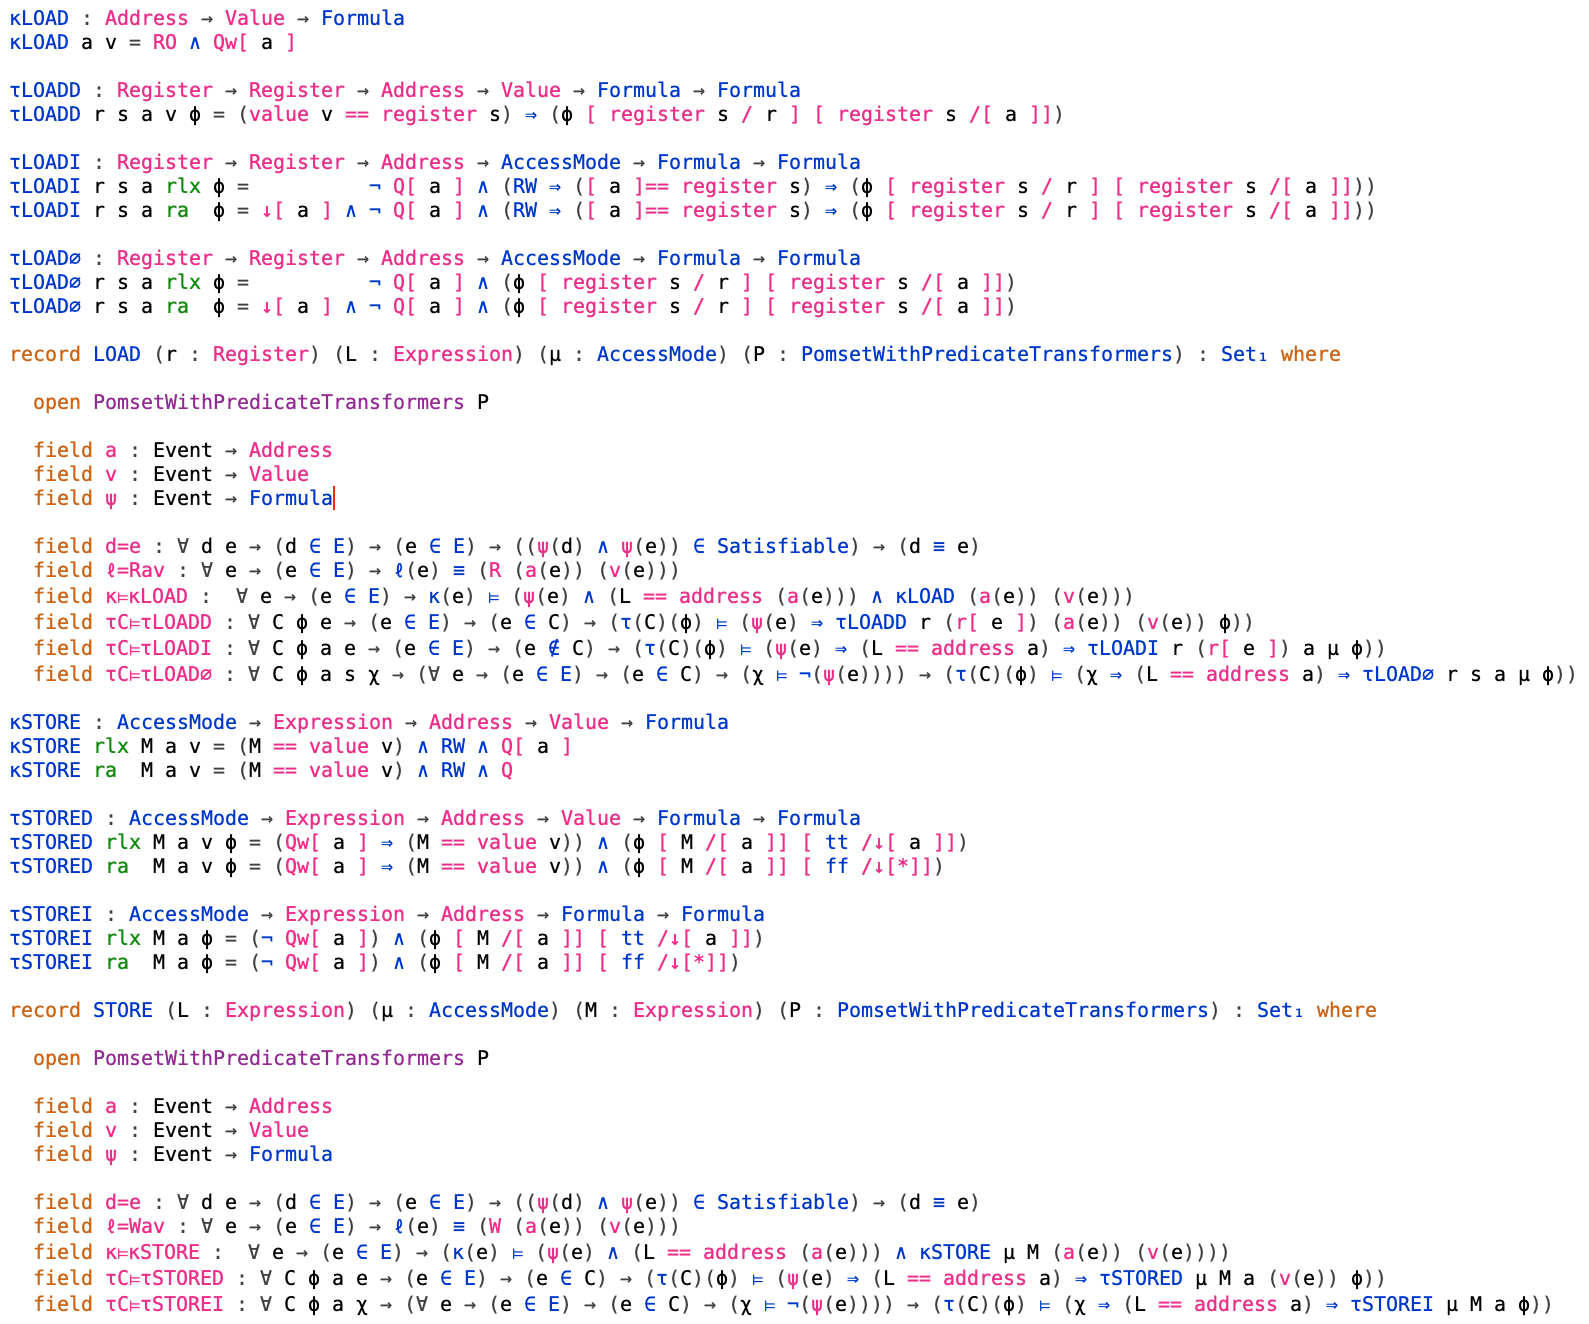
\includegraphics[width=\textwidth]{agda.png}
% \end{figure*}
